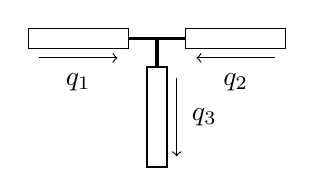
\begin{tikzpicture}
\draw (-1,0) node[rectangle,draw,minimum width=.5in,minimum height=.1in] (a) {};
\draw[->] (a) ++(-.5,-.25) -- node[pos=.5,below=2pt] {$q_{1}$} ++(1,0);
\draw (1,0) node[rectangle,draw,minimum width=.5in,minimum height=.1in] (e) {};
\draw[<-] (e) ++(-.5,-.25) -- node[pos=.5,below=2pt] {$q_{2}$} ++(1,0);
\draw (0,-1) node[rectangle,draw,minimum width=.1in,minimum height=.5in] (f) {};
\draw[<-] (f) ++(.25,-.5) -- node[pos=.5,right=2pt] {$q_{3}$} ++(0,1);
\draw[very thick] (a.0) |- (e.180);
\draw[very thick] (f.90) |- (e.180);
\end{tikzpicture}